% vim:ft=tex:
%
\documentclass{beamer}
\usepackage{graphicx}
\usepackage{listings}
\usepackage{verbatim}
\usepackage{tikz}

\let\oldfootnotesize\footnotesize

\lstset{
	basicstyle=\oldfootnotesize\ttfamily,
	escapeinside={\%*}{*)}
}

\newcommand\myheading[1]{%
  \par
  {\bfseries#1}\par}

\setbeamertemplate{footline}[]{}
\setbeamertemplate{navigation symbols}{}


\title{
	Denial of Service Attacks
}
\author{
	Andrew DeMaria (muff1nman) --- \texttt{ademaria@mines.edu}
}

\begin{document}
\maketitle

{
	\begin{frame}[plain]
		\begin{tikzpicture}[remember picture,overlay]
			\node[at=(current page.center)] {
				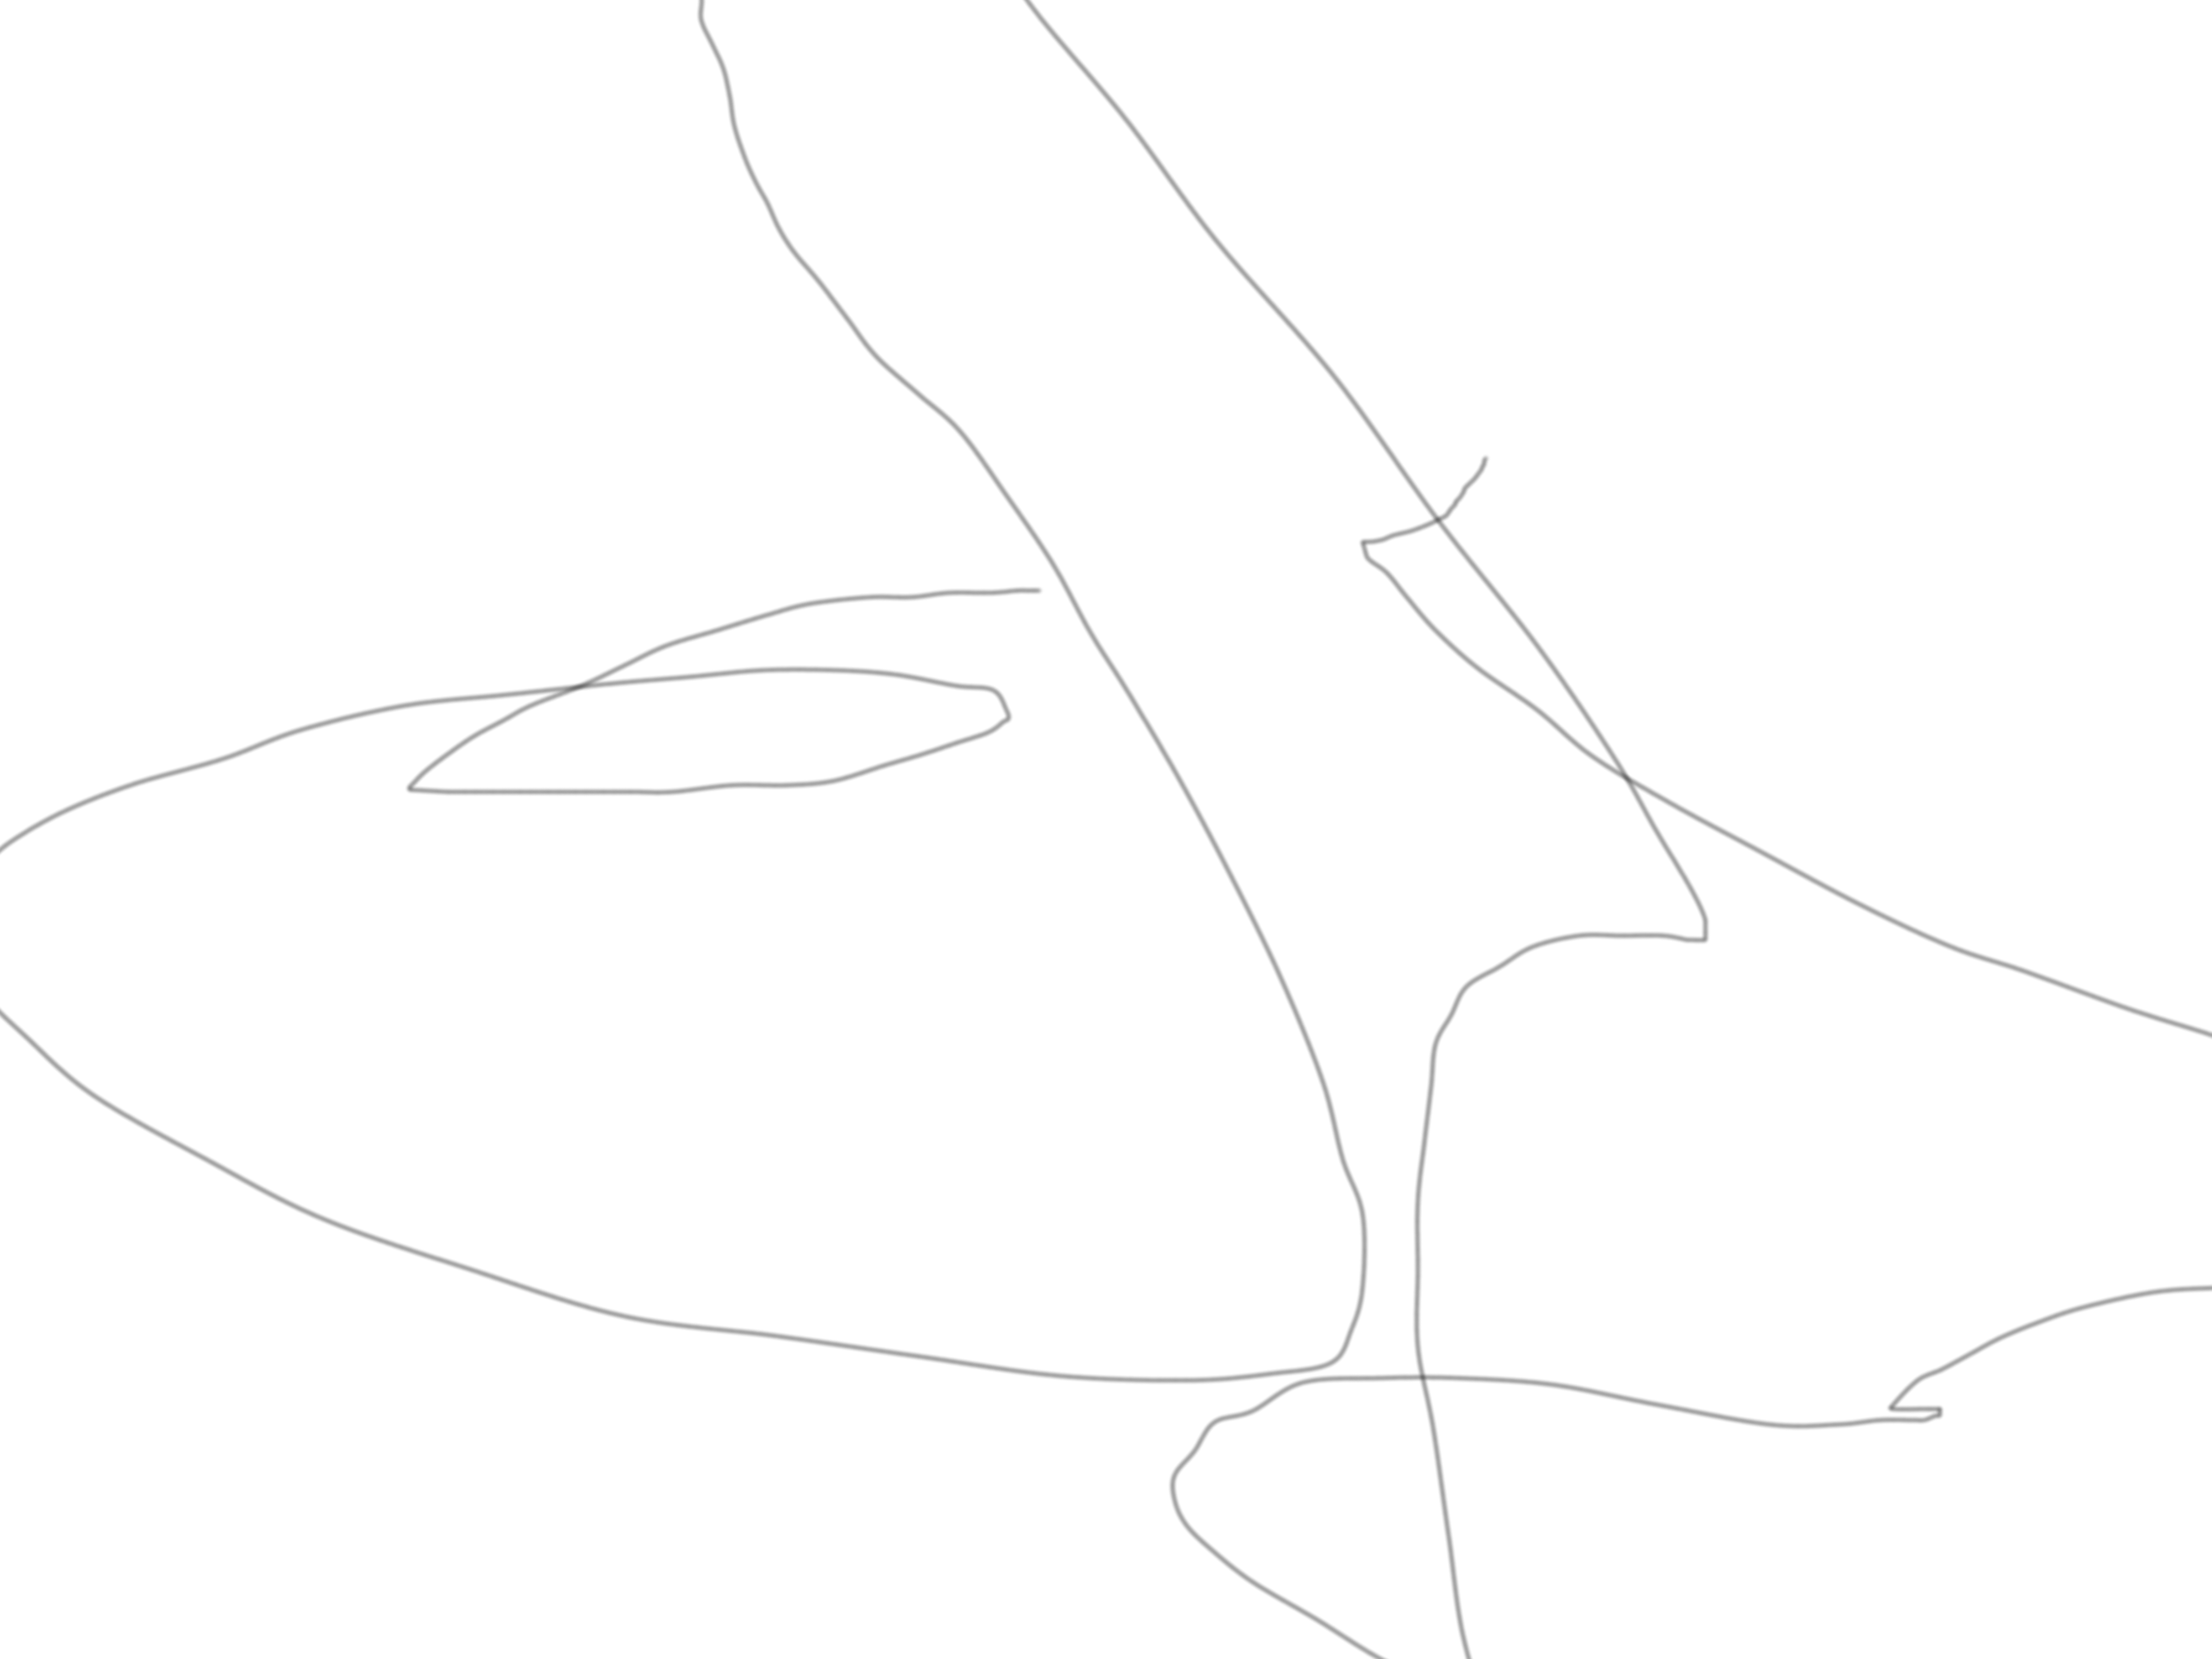
\includegraphics[width=\paperwidth]{images/Collage.png}
			};
		\end{tikzpicture}
	\end{frame}
}

\begin{frame}[allowframebreaks,t]{Agenda}
	\begin{itemize}
		\item Background
			\begin{itemize}
				\item OSI model
			\end{itemize}
		\item{SYN Floods}
		\item{DNS Reflection}
		\item{r-u-dead-yet? (RUDY)}
	\end{itemize}
\end{frame}

\begin{frame}{OSI Model}
	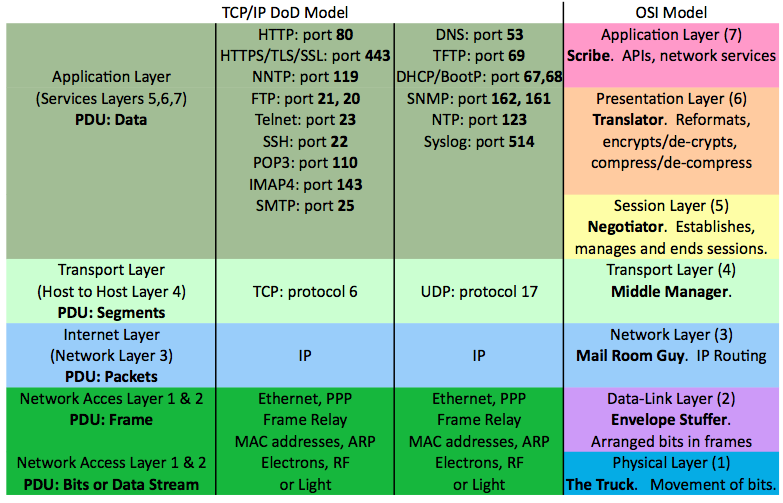
\includegraphics[width=\textwidth]{images/osi2.png}
\end{frame}

\begin{frame}{SYN Flood}
	%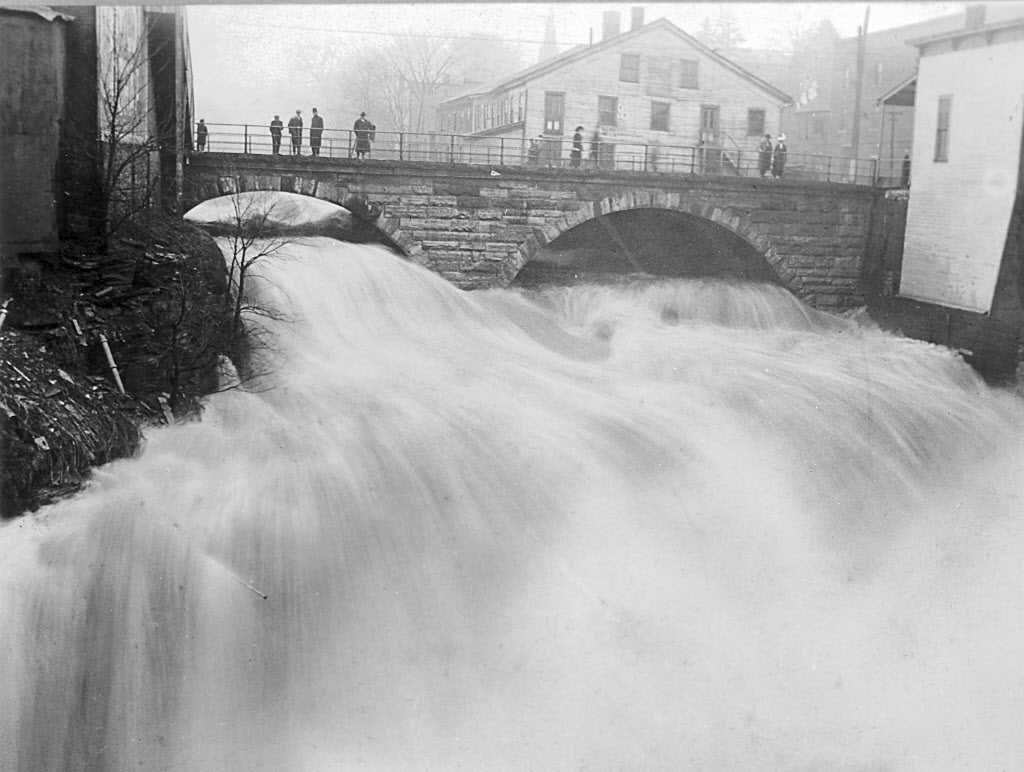
\includegraphics[width=1\textwidth]{images/flood.jpg}
	\begin{center}
		\vspace*{\fill}
		{\Large SYN Flood}
		\vspace*{\fill}
	\end{center}
\end{frame}

\begin{frame}
	\frametitle{SYN Flood... Background}
	\framesubtitle{TCP's Handshake process}
	\begin{itemize}
		\item TCP, or Transmission Control Protocol is a Layer 2 protocol underlying
			most internet communications today.  It uses a 3 step handshake to
			establish a connection
			\begin{enumerate}
				\item Client will send a $SYN$ to a listening server.  The sequence
					number($seq\_num$) is set to a random number.
				\item Server responds with $SYN$-$ACK$, with the acknowledgement number
					($ack\_num$) set to 1 plus the $seq\_num$.  It sets a new random value
					for $seq\_num$
				\item Client responds with an $ACK$.
					\begin{itemize}
						\item $ack\_num = 1 + seq\_num$
						\item $seq\_num = 1 + ack\_num$
					\end{itemize}
			\end{enumerate}
	\end{itemize}
\end{frame}

\begin{frame}
	\frametitle{SYN Flood... Theory}
	\only<1>{
	\framesubtitle{The flaw in TCP}
	\begin{itemize}
		\item The TCP handshake process requires the server to save
			state before the connection can be established
			\begin{itemize}
				\item Sequence and Acknowledgement numbers need to be saved
				\item State is saved in a Transmission Control Block (TCB)
			\end{itemize}
		\item There is a limited amount of room that the operating system saves for
			TCBs 
	\end{itemize}
}
\only<2>{
	\framesubtitle{Attack Steps}
	\begin{enumerate}
		\item The attacker sends a $SYN$ packet
		\item The victim sends back a $SYN$-$ACK$
			% The attacker may also spoof the ip address so that his machine does not
			% respond and close the connection
		\item The attacker sends... {\em nothing}
		\item This leaves a half open TCP connection on the server, consuming
			resources
		\item Attacker repeats Step 1 many times
			\begin{itemize}
				\item TCP connections are only flushed out after a period of time, or in
					some implementations, when the TCB pool is depleted
			\end{itemize}
		\item With so many open connections on the server, new legitimate traffic
			cannot get through
	\end{enumerate}
}
\end{frame}

\begin{frame}
	\frametitle{SYN Flood... Demo}
	\begin{center}
		\vspace*{\fill}
		{\Large Demo}
		\vspace*{\fill}
	\end{center}
\end{frame}

\begin{frame}
	\frametitle{SYN Flood... Mitigations}
	\begin{itemize}
		\item SYN Caching
			\begin{itemize}
				\item Instead of creating an entire TCB, use a table for half-open
					connections
			\end{itemize}
		\item SYN Cookies
			\begin{itemize}
				\item Lazily creates TCBs so that half open connections don't require
					resources %TODO
			\end{itemize}
		\item Application Firewalls / Proxy
			\begin{itemize}
				\item Lets an external system do all the TCP connection management and
					forwards completed connections along
			\end{itemize}
	\end{itemize}
\end{frame}

\begin{frame}{DNS Reflection Attacks}
	\begin{center}
		\vspace*{\fill}
		{\Large DNS Reflection Attacks}
		\vspace*{\fill}
	\end{center}

\end{frame}

\begin{frame}[fragile]
	\frametitle{DNS Reflection Attacks... Background}
	\only<1>{
		\framesubtitle{What is DNS?}
		\begin{itemize}
			\item DNS (Domain Name System) provides a mapping of names to IP addresses
				%That way we can keep down on the number of mysql ip addresses we have to
				%memorize :)
			\begin{semiverbatim}
			www.google.com -> 74.125.227.112
			\end{semiverbatim}

			\item DNS Servers / Nodes can have several different types of records
				%for which they are authoritative
				\begin{itemize}
					\item {\ttfamily A} % The typical ip record
					\item {\ttfamily CNAME}
						% For any aliases that also map to the A record.
					\item {\ttfamily AAAA} 
						% ip 6
					\item {\ttfamily TXT}	\dots
				\end{itemize}
			\item DNS has a hierarchal structure with authoritative nodes
			\item Clients / Resolvers iteratively query DNS servers
				\begin{itemize}
					\item A resolver seeking "www.google.com" starts at "root", then
						"com", "google", \dots
				\end{itemize}
			\item Queries use UDP %\em{important}
		\end{itemize}
	}
\end{frame}

\begin{frame}
	\frametitle{DNS Reflection Attacks... Theory}
	\framesubtitle{The Theory behind the Attack}
	The idea behind a DNS reflection attack is to make large DNS requests on
	behalf of your victim
	\begin{enumerate}
		\item The attacker sends queries, spoofing the victim's IP, to many
			different DNS servers
			\begin{itemize}
				\item Remember.. this is UDP
			\end{itemize}
			% As compared to TCP where a handshake would be involved
		\item DNS server responses are sent to the victim
		\item Attack generates so much traffic that the hardware can't even keep up
			%10 Gpbs up is saturated by a 11 Gpbs down
	\end{enumerate}
	However... None of this is possible without open DNS resolvers...
\end{frame}

\begin{frame}[fragile]
	\frametitle{DNS Reflection Attacks... Open Resolvers}
	\only<1>{
		\framesubtitle{What are Open Resolvers?}
		Open Resolvers are misconfigured DNS servers that will respond to recursive
		requests for domains they are not authoritative for.
		\begin{itemize}
			\item To be authoritative, the domain must be in that DNS
				server's zone
			\item Normally DNS queries use an iterative approach
			\item Instead of pointing a query to the next domain, an open resolver
				makes the recursive requests on behalf of the requester
			%\item  It is okay for DNS servers to be recursive.  The caching servers setup by
				%your ISP are recursive, but only for requests coming from their zone. 
			%\item The problem lies when anyone can make a query to an open resolver
		\end{itemize}
	}
\end{frame}

\begin{frame}
	\frametitle{DNS Reflection Attacks... Demo}
	\begin{center}
		\vspace*{\fill}
		{\Large Demo}
		\vspace*{\fill}
	\end{center}
\end{frame}

\begin{frame}
	\frametitle{DNS Reflection Attacks... Open Resolvers}
		\framesubtitle{So how bad is it?}
		There are a little over 28 {\em million} open resolvers operating
		today\footnote{ As reported by http://openresolverproject.org/breakdown.cgi on
		2013-08-11}
		\begin{itemize}
			\item It is pretty trivial for attackers to find them
			\item Most businesses / organizations don't even realize that they are
				contributing to the demise of the internet
		\end{itemize}
\end{frame}

\begin{frame}
	\frametitle{DNS Reflection Attacks... Increasing the effectiveness}
	\framesubtitle{DNS Reflection attacks can be further amplified }
	\begin{itemize}
		\item Botnets allow for additional throughput on the attackers size,
			linearly scaling the attack
		\item Extensions to DNS allow for increase response size
			\begin{itemize}
				\item EDNS 0 allows for DNS packets to go beyond the initial 512 byte
					limit up to 4096 bytes
				\item DNSSEC adds fields for keys and signatures for validating DNS
					records
			\end{itemize}
		\item Attackers may also compromise a DNS server to publish their own
			records
	\end{itemize}
\end{frame}

\begin{frame}
	\frametitle{DNS Reflection Attacks... Mitigation}
	\begin{itemize}
		\item Shutdown all the open resolvers
			\pause
		\item realistically...
			\pause
			Get yourself a good third party hosting service
			\pause
		\item Third party companies such as Cloudflare specialize in hosting customers
			content and thwarting DNS Reflection attacks
		%\item Web Application Firewalls will not save you here {\em that's not to
			%say they are useless} 
	\end{itemize}
\end{frame}

\begin{frame}
	\frametitle{r-u-dead-yet?}
\end{frame}

\begin{frame}
	\frametitle{r-u-dead-yet?}
	\framesubtitle{Not all DOS attacks require high volume traffic}
	\begin{itemize}
		\item RUDY (r-u-dead-yet?) is a low-volume DOS attack that utilizes HTTP
			POST forms on a webservice
		\item Instead of sending full packets for the POST data, it sends the data a
			byte at a time, with long time intervals between data segments
		\item The webserver's connection pool becomes used up as all the threads are
			waiting on incoming POST data
		% \item  unique in that all packets are legal and has a very low volume TODO
	\end{itemize}
\end{frame}

\begin{frame}
	\frametitle{r-u-dead-yet?}
	\framesubtitle{The issue and a fix}
	\begin{itemize}
		\item Apache was vulnerable to this attack up to version 2.2 
			\begin{itemize}
				\item Apache would keep connections open for 300 seconds (5 min)!
			\end{itemize}
		\item Now most webservers allow users to specify a value for
			{\ttfamily ReadRequestTimeout} to ensure a quicker turn around time for
			threads  (30 seconds for Apache)
	\end{itemize}
\end{frame}

\begin{frame}
	\frametitle{Questions?}
	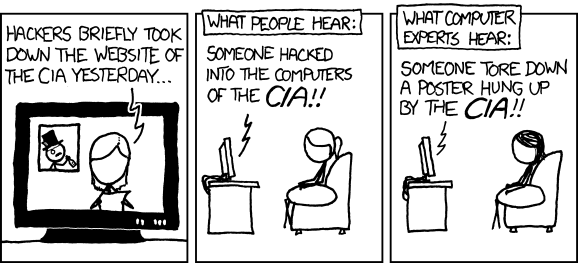
\includegraphics[width=1\textwidth]{images/cia.png}
	\newline
	{\footnotesize Image source: http://xkcd.com/932/}
\end{frame}
\end{document}

